\chapter{Huấn luyện mạng nơ-ron nhiều tầng ẩn bằng thuật toán Adam}
\label{Chapter3}

\textit{Chương này trình bày về thuật toán tối ưu Adam và cách thuật toán khắc phục khó khăn trong huấn luyện mạng nơ-ron nhiều tầng ẩn mà khoá luận tập trung tìm hiểu. Đầu tiên chúng tôi trình bày về các thuật toán nền tảng: (1) thuật toán Gradient Descent với Momentum để tăng tốc và giảm dao động trong quá trình di chuyển trên bề mặt lỗi, và (2) thuật toán Gradient Descent với tỉ lệ học thích ứng với từng trọng số, cụ thể là thuật toán Adagrad và RMSprop. Dựa trên nền hai thuật toán này, chúng tôi trình bày ý tưởng của thuật toán Adam cũng như những ưu/khuyết điểm của thuật toán trong giải quyết các khó khăn của bài toán huấn luyện mạng nơ-ron.}

\section{Thuật toán Gradient Descent với Momentum}

Các thuật toán sử dụng gradient như GD và SGD gặp phải hai khó khăn chính khi chỉ có thông tin của véc-tơ gradient mà thiếu đi thông tin về độ cong của bề mặt lỗi. Đầu tiên, vì hướng của gradient là hướng có độ dốc lớn nhất nên không phải lúc nào cũng là hướng tốt nhất và có thể gây dao động mạnh trong khi độ lỗi giảm không nhiều. Thứ hai, ``độ nhạy cảm'' của mỗi trọng số là khác nhau trong bề mặt lỗi, vì vậy áp dụng một tỷ lệ học chung cho tất cả các trọng số sẽ khiến cho hướng cập nhật bỏ qua các trọng số có ``độ nhạy cảm'' nhỏ.

``GD/SGD với Momentum'' (hay ``Momentum'') đều được dùng để chỉ một phương pháp cải tiến sử dụng quán tính để điều chỉnh hướng gradient theo hướng tốt nhất về cực tiểu, từ đó tăng tốc độ di chuyển trên bề mặt lỗi. Quán tính được thêm vào công thức thông qua hệ số quán tính $\beta$ được chọn trước khi trình huấn luyện và công thức cập nhật $\theta$ tại mỗi bước được cải tiển như công thức \ref{eqn:theta-momentum}. Dưới góc nhìn vật lý, Momentum trong công thức \ref{eqn:vt} là phần vận tốc còn lại sau khi tiêu hao trong quá trình vật di chuyển về vị trí cân bằng, quyết định mức độ dao động và tốc độ di chuyển của vật. Với một hệ số momentum càng cao, lượng vận tốc tiêu hao càng ít, vận tốc càng lớn thì lượng dao động của vật càng nhiều khiến cho vật mất nhiều thời gian để trở về vị trí cân bằng. Ngược lại, nếu hệ số momentum quá thấp, lượng vận tốc tiêu hao quá lớn dẫn đến vật không thể đến vị trí cân bằng. Tương tự như vậy, trong huấn luyện mạng nơ-ron, một hệ số momentum quá cao sẽ khiến cho hướng di chuyển bị dao động nhiều quanh điểm cực tiểu nhưng không thể hội tụ, và ngược lại, thời gian huấn luyện sẽ tăng lên đáng kể.

\begin{equation}
	\label{eqn:vt}
	v_t = \beta v_{t-1} + \alpha \nabla E(\theta_t)
\end{equation}

\begin{equation}
	\label{eqn:theta-momentum}
	\theta_t = \theta_{t-1} - v_t
\end{equation}

Có thể nói hệ số momentum điều chỉnh mức độ ``ghi nhớ'' của thuật toán. Hệ số momentum càng lớn thì giá trị quán tính cũ được ghi nhớ càng lâu và ngược lại. Điều đó liên quan đến đường trung bình động hàm mũ (Exponential Moving Averages) hay EMA. Đường trung bình động hàm mũ cho phép ta sử dụng trung bình động để xử lý nhiễu trong dữ liệu mà ta quan sát được và xấp xỉ nó gần hơn với dữ liệu thực. Ta thực hiện lấy trung bình trên $\frac{1}{1-\beta}$ bước nhảy gần nhất và thực hiện cập nhật trọng số. Ta khai triển công thức \ref{eqn:vt} như sau:

\begin{equation}
	\label{eqn:v3}
	\begin{aligned}
		v_1 &= \beta v_0 + \alpha\nabla E(\theta_1) \\
		v_2 &= \beta v_1 + \alpha \nabla E(\theta_2) = \beta (v_0 + \alpha\nabla E(\theta_1)) + \alpha\nabla E(\theta_2) \\
		&= \beta v_0 + \beta\alpha\nabla E(\theta_1) + \alpha\nabla E(\theta_2) \\
		v_3 &= \beta v_2 + \alpha\nabla E(\theta_3) = \beta (\beta v_0 + \beta\alpha\nabla E(\theta_1) + \alpha\nabla E(\theta_2)) + \alpha\nabla E(\theta_3) \\
		&= \beta^2 v_0 + \beta^2\alpha \nabla E(\theta_1) + \beta \alpha \nabla E(\theta_2) +\alpha \nabla E(\theta_3)
	\end{aligned}
\end{equation}

Từ công thức \ref{eqn:v3} ta nhận thấy rằng tại bước nhảy thứ $t$, giá trị của momentum phụ thuộc vào tất cả các giá trị momentum trước đó từ $1..(t-1)$. Mỗi giá trị trong dãy đều được nhân với hệ số $\beta^t$. Vì $\beta$ là hệ số quán tính nằm trong khoảng $(0,1)$ nên $\beta^t$ sẽ càng nhỏ khi $t$ càng lớn dẫn đến các giá trị càng lâu trước đó sẽ có hệ số càng nhỏ và dần không đóng góp gì nhiều trong quá trình huấn luyện. Hay nói cách khác, các giá trị này dần được quên đi và thuật toán Momentum quan tâm nhiều đến các giá trị gần với hiện tại.

Trong thực tế huấn luyện, ta thường sử dụng cách xấp xỉ true gradient bằng các gradient của tập con để tăng tốc quá trình cập nhật trọng số. Trong quá trình xấp xỉ, việc tạo minibatch bằng cách gom nhóm ngẫu nhiên các điểm dữ liệu đã thêm một lượng nhiễu vào trong quá trình tối ưu. So sánh độ lớn của nhiễu với độ lớn của momentum ta có thể chia quá trình thành hai giai đoạn: giai đoạn ``transient'' và giai đoạn ``fine-tuning''. Trong giai đoạn transient, momentum vẫn còn hiệu quả trong điều chỉnh hướng của gradient và giúp gradient tiến nhanh về vị trí có cực tiểu vì độ lớn của momentum lớn hơn độ lớn của nhiễu. Quá trình huấn luyện càng lâu, độ lớn của momentum ngày càng giảm và bị lấn át bởi độ nhiễu, khi đó ta bước qua giai đoạn fine-tuning. Trong các mạng nơ-ron nhiều tầng ẩn, giai đoạn fine-tuning chiếm một phần ít hơn và cũng ít quan trọng hơn giai đoạn transient nên việc đảm bảo giai đoạn transient được diễn ra đủ lâu là một sự cần thiết \cite{sutskever2013onti}.

Sự chuyển đổi giữa hai quá trình được kể trên được quyết định bởi hằng số quán tính $\beta$. Sử dụng một hệ số quán tính $\beta$ lớn cho phép momentum thực hiện quá trình tối ưu tốt hơn trên các hướng có ``độ nhạy cảm'' nhỏ. Tuy nhiên, lợi thế này không được thể hiện qua rõ ràng qua độ lỗi do thuật toán không thể hội tụ tốt tại các hướng có ``độ nhạy cảm'' cao với một hệ số quán tính $\beta$ lớn. Sự đánh đổi này cho kết quả là ta có thể tiến gần đến vùng có cực tiểu hoặc là hội tụ tại cực tiểu có độ lỗi nhỏ hơn. Trong khi sử dụng một hệ số $\beta$ nhỏ sẽ cho độ lỗi cao hơn vì giai đoạn transient kết thúc quá sớm. Thiếu đi sự hỗ trợ của momentum, các phương pháp bậc nhất không thể tận dụng tốt thông tin tại các hướng có ``độ nhạy cảm'' nhỏ và rất dễ bỏ qua các vùng chứa cực tiểu hoặc cực tiểu có độ lỗi thấp hơn dẫn đến hội tụ tại điểm có độ lỗi cao.

\begin{figure}[htp]
	\centering
	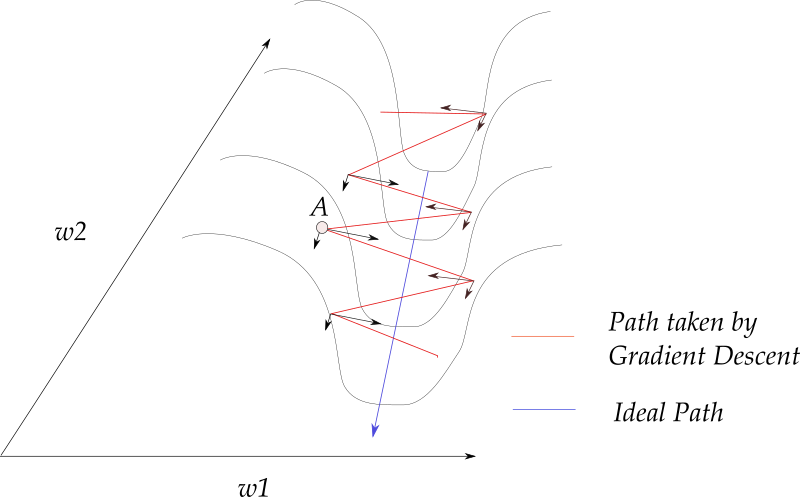
\includegraphics[width=140 mm]{images/valley-momentum.png}
	\caption{Minh họa cách Momentum triệt tiêu hướng có độ dốc lớn. (Nguồn: \url{https://blog.paperspace.com/intro-to-optimization-momentum-rmsprop-adam/})}
	\label{fig:valley-momentum}
\end{figure}

Đặc biệt trong trường hợp rãnh hẹp, momentum giúp GD/SGD tăng tốc độ hội tụ đáng kể. Ta có thể thấy trong Hình \ref{fig:valley-momentum}, tại một điểm $A$ bất kỳ, ta có thể phân tích thành hai véc-tơ thành phần của từng trọng số. Vì rãnh hẹp nên sẽ có một hướng có độ dốc cao hơn hướng còn lại, trong trường hợp này là $w_1$, nên độ dài véc-tơ tương ứng tại hướng đó sẽ có độ dài lớn hơn độ dài véc-tơ tại hướng còn lại. Thuật toán GD/SGD sẽ ưu tiên hướng có độ dốc cao hơn và bỏ qua hướng $w_2$ có độ dốc thấp, gây ra hiện tượng dao động cho độ lỗi giảm ít với thời gian huấn luyện lâu. Một giải pháp thường được sử dụng để khắc phục hiện tượng này là giảm tỉ lệ học của thuật toán GD/SGD. Tuy nhiên, để khắc phục hiện tượng dao động, ta cần một tỉ lệ học rất nhỏ, với tỉ lệ học này thuật toán GD/SGD sẽ không thể ``khám phá'' những hướng có độ dốc nhỏ một cách hiệu quả do tốc độ giá trị gradient biến đổi tại những hướng này là rất chậm và dễ dàng bị lấn át bởi hướng có độ dốc cao. Trong trường hợp hướng đi về cực tiểu là một trong các hướng có độ dốc thấp, thuật toán GD/SGD sẽ thực hiện những bước cập nhật rất nhỏ, cho cảm giác huấn luyện bị chững lại và tạo cảm giác gặp phải cực tiểu địa phương.

Momentum giải quyết vấn đề này bằng cách cộng dồn các véc-tơ quán tính. Khi cộng dồn, các véc-tơ tại hướng có độ dốc lớn $w_1$ sẽ bị triệt tiêu và véc-tơ tại hướng có độ dốc nhỏ $w_2$ được tăng cường. Từ đó, momentum giúp điều chỉnh hướng của gradient và tăng tốc độ hội tụ của thuật toán.

\section{Thuật toán Gradient Descent với tỉ lệ học thích ứng}

Việc dự đoán trong học máy nói chung và mạng nơ-ron nhiều tầng ẩn nói riêng dựa vào quá trình trích xuất và liên hệ các đặc trưng của dữ liệu. Thông thường, các điểm dữ liệu trong cùng một bài toán sẽ có những đặc trưng chung thường gặp. Tuy nhiên, cũng có một số đặc trưng rất hiếm khi xuất hiện, chỉ có ở trong một số ít điểm dữ liệu cụ thể. Các đặc trưng hiếm gặp này thường sẽ có ảnh hưởng rất lớn về mặt ý nghĩa của dữ liệu, và mang lại rất nhiều thông tin về điểm dữ liệu đó\cite{salton1988term}. Một ví dụ cụ thể là trong phân tích văn bản, các từ xuất hiện thường xuyên như các liên từ (``và'', ``thì'', ``nhưng'',...) hay các phó từ (``cũng'', ``lại'', ``rồi'',...) lại không thể hiện nội dung nhiều bằng các danh từ và động từ chỉ các đối tượng, hành động cụ thể. Một trường hợp khác là khi xét riêng một đặc trưng, những điểm dữ liệu mang giá trị khác với các điểm dữ liệu còn lại đóng vai trò quan trọng hơn trong việc cung cấp thông tin để giải quyết bài toán.

Tuy nhiên, các thông tin quan trọng được biểu diễn bằng các đặc trưng hiếm lại ít được mạng nơ-ron nhiều tầng ẩn chú ý. Trong mạng nơ-ron nhiều tầng ẩn, các nơ-ron tương ứng với các đặc trưng thường gặp sẽ được cập nhật thường xuyên, trong khi các nơ-ron tương ứng với các đặc trưng hiếm chỉ được cập nhật một số ít lần trong một lần duyệt qua toàn tập dữ liệu. Hiện tượng này khiến cho các đặc trưng thường gặp và mang ít thông tin được biểu diễn tốt hơn, còn các đặc trưng hiếm mang nhiều ý nghĩa lại chưa được học.

Mặc dù SGD và Momentum thực hiện cập nhật một lượng khác nhau cho mỗi trọng số tùy theo độ lớn của gradient tại điểm đang xét (và trạng thái của momentum tại thời điểm đó), tuy nhiên lượng cập nhật vẫn chỉ dựa vào hướng và độ dốc của gradient, hay nói cách khác là độ dốc của bề mặt lỗi, tại điểm đang xét và chưa tính tới độ nhạy cảm của các trọng số. John Duchi, Elad Hazan, và Yoram Singer đã đề xuất thuật toán Adagrad\cite{duchi2011adaptive} lấy ý tưởng từ phương pháp Newton để giải quyết vấn đề này bằng cách thích ứng lượng cập nhật cho từng trọng số: các trọng số tương ứng với các đặc trưng thường gặp sẽ được cập nhật ít hơn, còn các trọng số tương ứng với các đặc trưng hiếm sẽ được cập nhật lượng lớn hơn.

\begin{itemize}
	\item Từ khai triển Taylor ở công thức \ref{eqn:taylor-f}, chúng ta có thể tạo được một xấp xỉ bậc hai $\rho$ của hàm $f$ cho các giá trị $x$ xung quanh một điểm $x_0$:
	\begin{equation}
		\label{eqn:quad-approx}
		f(x) \approx \rho(x) = f(x_0) + f'(x_0) \cdot (x - x_0) + \frac{1}{2} \cdot f''(x_0) \cdot (x - x_0)^2
	\end{equation}
	\begin{figure}[H]
		\centering
		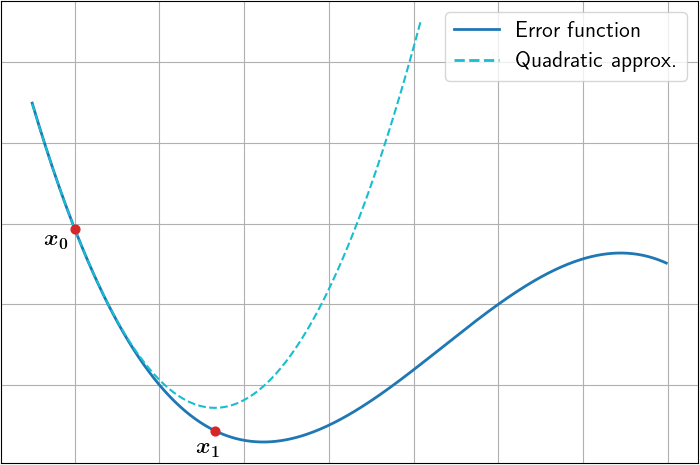
\includegraphics[width=120 mm]{images/quad-approx.png}
		\caption{Xấp xỉ bậc hai (đường đứt khúc màu xanh nhạt) của hàm lỗi (đường màu xanh đậm) và bước cập nhật tiếp theo của phương pháp Newton.}
		\label{fig:newton-step}
	\end{figure}
	Vì đây là một xấp xỉ bậc hai nên chúng ta có thể tìm cực trị của xấp xỉ này bằng cách giải phương trình $\rho '(x) = 0$. Khi đó nghiệm của $\rho'(x)$ sẽ là bước cập nhật tiếp theo của phương pháp Newton (hình~\ref{fig:newton-step}) được tính bằng công thức \ref{eqn:newton-update}:
	\begin{equation} \label{eqn:newton-update}
		\begin{aligned}
			\rho'(x_{t+1}) &= 0 \\
			\Rightarrow f'(x_t) + f''(x_t) \cdot (x_{t+1} - x_t) &= 0 \\
			\Rightarrow x_{t+1} &= x_t - \frac{f'(x_t)}{f''(x_t)}
		\end{aligned}
	\end{equation}

	\item Ma trận Hessian là ma trận vuông gồm các đạo hàm bậc hai theo từng cặp hướng của một hàm số. Cho một hàm số $f$ có tham số đầu vào là một véc-tơ $x \in \mathbb{R}^M$, chúng ta sẽ có ma trận vuông Hessian $H$ kích thước $M\times M$ theo công thức:
	\begin{equation}
		H = \begin{bmatrix}
			\frac{\delta^2 f}{\delta x^{2}_1} & \frac{\delta^2 f}{\delta x_1 \delta x_2} & \dotsb & \frac{\delta^2 f}{\delta x_1 \delta x_M} \\
			\frac{\delta^2 f}{\delta x_2 \delta x_1} & \frac{\delta^2 f}{\delta x^{2}_2} & \dotsb & \frac{\delta^2 f}{\delta x_2 \delta x_M} \\
			\vdots & \vdots & \ddots & \vdots \\
			\frac{\delta^2 f}{\delta x_M \delta x_1} & \frac{\delta^2 f}{\delta x_M \delta x_2} & \dotsb & \frac{\delta^2 f}{\delta x^{2}_M}
		\end{bmatrix}
	\end{equation}

	\item Để khái quát hóa phương pháp Newton cho bài toán tối ưu trong không gian cao chiều, ta thay đạo hàm bậc nhất và đạo hàm bậc hai từ công thức \ref{eqn:quad-approx} lần lượt bằng gradient $g(x_0)$ và ma trận Hessian $H$ tại điểm $x_0$:
	\begin{equation} \label{eqn:hessian-approx}
		f(x) \approx \rho(x) = f(x_0) + g(x_0)^\top (x - x_0) + \frac{1}{2}(x - x_0)^\top H(x - x_0)
	\end{equation}
	Tương tự như trên, chúng ta cũng giải phương trình $\nabla\rho(x)=0$ để tìm bước cập nhật tiếp theo:
	\begin{equation} \label{eqn:hessian-update}
		\begin{aligned}
			\nabla \rho(x_t) &= 0 \\
			\Rightarrow g(x_t) + H_t \cdot (x_{t+1} - x_t) &= 0 \\
			\Rightarrow x_{t+1} &= x_t - H^{-1}_t \cdot g(x_t)
		\end{aligned}
	\end{equation}
\end{itemize}

Tại mỗi bước cập nhật, phương pháp Newton xấp xỉ bề mặt lỗi xung quanh điểm hiện tại bằng một parabol $P$ có cùng độ dốc và độ cong với bề mặt lỗi tại điểm đang xét. Từ đó, bước cập nhật trong công thức \ref{eqn:hessian-update} sẽ cho một điểm mới là điểm cực trị trong parabol $P$ (cực tiểu nếu parabol $P$ có bề lõm quay lên trên; cực tiểu nếu parabol $P$ có bề lõm quay xuống dưới). Ví dụ một hàm số bậc hai có dạng $y_1 = ax^2 + bx + c$ sẽ có đồ thị là một parabol $P_1$ có bề lõm hướng lên và điểm cực tiểu là điểm $A(\frac{-b}{2a};\frac{-\Delta}{4a})$. Lấy một điểm B bất kỳ thuộc parabol $P_1$ có toạ độ $(x_B,y_B)$ với $x_B > \frac{-b}{2a}$. Để từ $B$ đến được cực tiểu $A$ trong một bước, thì tạo độ điểm $B$ phải thay đổi một lượng $\Delta x = x_B - x_A = x_B + \frac{b}{2a} = \frac{2ax_B + b}{2a} = \frac{f'(x_B)}{f''(x_B)}$. Vậy từ điểm $B$ ta thực hiện bước cập nhật $x_B - \Delta x$ thì ta đến được điểm $A$. Trong trường hợp hàm nhiều biến, đạo hàm bậc nhất $f'(x_B)$ sẽ được thay bằng véc-tơ gradient và đạo hàm bậc hai sẽ được thay bằng ma trận Hessian. Viết lại theo dạng tổng quát ta sẽ được công thức \ref{eqn:hessian-update}. Vì vậy các thuật toán bậc hai bị "thu hút" bởi các điểm cực trị dẫn đến mắc kẹt tại điểm yên ngựa. Đồng thời đây là một trong những lý do quan trọng khiến các phương pháp bậc hai ít được sử dụng hơn các phương pháp bậc nhất trong huấn luyện mạng nơ-ron nhiều tầng ẩn. Các phương pháp bậc nhất không gặp vấn đề này do hướng của gradient là hướng có độ thay đổi lớn nhất, đồng nghĩa với việc hướng gradient luôn chỉ về cực đại. Bằng cách đi ngược lại với hướng của gradient, ta luôn có thể tìm về một điểm mới có độ lỗi nhỏ hơn điểm hiện tại. Vấn đề của các phương pháp bậc nhất gặp phải là độ lớn bước cập nhật quá nhỏ. Các phương pháp tỉ lệ học thích ứng giúp thay đổi điều này bằng thông tin xấp xỉ được từ ma trận Hessian để thay đổi kích thước của bước cập nhật.

Ngoài ra, phương pháp Newton phụ thuộc khá lớn vào việc xấp xỉ cục bộ tại một điểm trên bề mặt lỗi. Vì vậy, một xấp xỉ không chính xác dễ dàng gây ra những bước cập nhật kém hiệu quả và có khả năng thuật toán không thể hội tụ tại cực tiểu. Các trường hợp này thường xảy ra khi các đạo hàm riêng bậc hai bằng 0 hoặc tiến gần về 0, khiến cho việc xấp xỉ bằng ma trận nghịch đảo không còn chính xác. Từ đó công thức \ref{eqn:hessian-update} cho ta một điểm mới có độ lỗi lớn hơn điểm hiện tại (hình \ref{fig:newton-bad-step}).

\begin{figure}
	\centering
	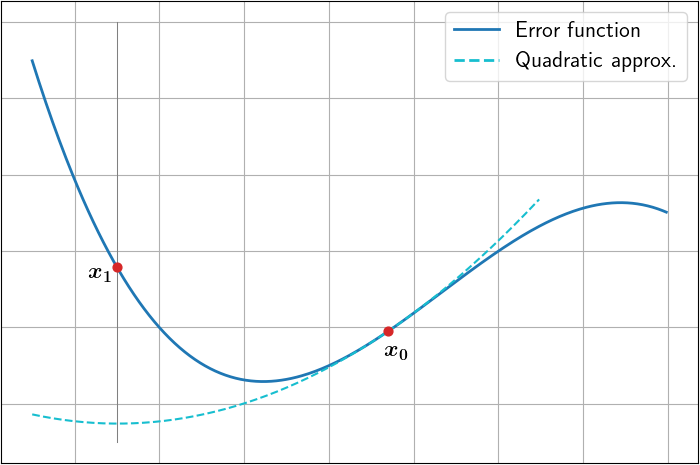
\includegraphics[width=120 mm]{images/hessian-osc.png}
	\caption{Cực tiểu của xấp xỉ bậc hai cung cấp một bước cập nhật không tối ưu.}
	\label{fig:newton-bad-step}
\end{figure}

Một hạn chế khác của các phương pháp bậc hai như phương pháp Newton nằm ở việc tính toán ma trận Hessian. Trong không gian $\mathbb{R}^M$ với $M$ có thể lên tới hàng trăm triệu hay thậm chí là hàng tỷ tương ứng với số trọng số của mô hình, ma trận Hessian sẽ yêu cầu thời gian tính toán và bộ nhớ quá lớn, dẫn đến việc sử dụng các phương pháp bậc hai cho bài toán tối ưu mạng nơ-ron nhiều tầng ẩn là bất khả thi.

Thuật toán Adagrad cũng sử dụng nguyên lý xấp xỉ bề mặt lỗi tương tự như phương pháp Newton. Tuy nhiên, thay vì tính trực tiếp ma trận Hessian nghịch đảo ($H^{-1}$, công thức \ref{eqn:hessian-update}), Adagrad chỉ thực hiện xấp xỉ tương đối $H^{-1}$ và tính bước cập nhật tiếp theo bằng công thức \ref{eqn:adagrad-base}:

\begin{equation}
	\label{eqn:adagrad-base}
	x_{t+1} = \prod^{diag(G_t)^{1/2}}_{X}(x_t-\eta\cdot diag(G_t)^{-1/2}\cdot g_t)
\end{equation}
với $g_t$ là véc-tơ gradient ở thời điểm $t$ và $G_t = \sum^{t}_{i=0}g_i\cdot g^{\top}_i$. Công thức \ref{eqn:adagrad-base} chỉ sử dụng gradient bậc nhất để xấp xỉ đường chéo của ma trận Hessian. Vì các bước tính đường chéo và căn bậc hai của ma trận $G_t$ có chi phí tuyến tính nên thuật toán Adagrad vẫn đảm bảo hiệu quả tính toán.

\begin{itemize}
	\item Vì gradient $g$ là một véc-tơ, biểu thức $g \cdot g^{\top}$ sẽ cho kết quả là một ma trận vuông kích thước $M \times M$ với mỗi phần tử là tích của từng cặp hướng trong véc-tơ gradient:
	\begin{equation} \label{eqn:grad-gradT}
		G = g \cdot g^{\top} = \begin{bmatrix}
			g^{2}_1 & g_1 \cdot g_2 & \dotsb & g_1 \cdot g_M \\ \\
			g_2 \cdot g_1 & g^{2}_2 & \dotsb & g_2 \cdot g_M \\
			\vdots & \vdots & \ddots & \vdots \\
			g_M \cdot g_1 & g_M \cdot g_2 & \dotsb & g^{2}_M
		\end{bmatrix}
	\end{equation}

	\item Từ kết quả công thức \ref{eqn:grad-gradT}, đường chéo của ma trận $G$ là véc-tơ $\begin{bmatrix} g^{2}_{1} & g^{2}_{2} & \cdots & g^{2}_{M} \end{bmatrix}$, hay bình phương của các giá trị đạo hàm riêng tại các hướng. Từ đó, ta có công thức tính $G_t$ \ref{eqn:adagrad-G} và bước cập nhật của thuật toán Adagrad được viết lại thành công thức \ref{eqn:adagrad-update}:
	\begin{equation} \label{eqn:adagrad-G}
		G_{t} = G_{t-1} + g^{2}_{t}
	\end{equation}
	\begin{equation} \label{eqn:adagrad-update}
		\theta_t = \theta_{t-1} - \frac{\eta}{\sqrt{G_t} + \epsilon} \cdot g
	\end{equation}
\end{itemize}

Tại mỗi bước cập nhật $t$, công thức \ref{eqn:adagrad-G} tính $G_t$ bằng cách cộng dồn bình phương của gradient theo từng hướng. Như vậy, các trọng số được cập nhật nhiều và thường xuyên sẽ có giá trị tương ứng trong $G_t$ lớn, trong khi các trọng số ít được cập nhật sẽ có giá trị nhỏ hơn. Do siêu tham số tỉ lệ học được chia cho căn bậc hai của $G_t$ (công thức \ref{eqn:adagrad-update}), nên tỉ lệ học của các trọng số có giá trị lớn trong $G_t$ bị tiêu giảm, đồng thời tăng cường tỉ lệ học cho các trọng số có giá trị trong $G_t$ nhỏ. Khả năng điều chỉnh tỉ lệ học tùy theo mức độ và tần suất cập nhật cho mỗi trọng số của Adagrad đã tạo ra nhóm phương pháp ``tỉ lệ học thích ứng''. Việc điều chỉnh tỉ lệ học cho từng trọng số giúp mô hình chú ý nhiều hơn đến các đặc trưng hiếm gặp của dữ liệu.

Tuy nhiên, do $g^{2}_{t}$ luôn luôn không âm nên giá trị của $G_t$ luôn luôn tăng dần, khiến cho tỉ lệ học bị giảm dần. Khi quá trình huấn luyện càng kéo dài, tỉ lệ học sẽ bị suy biến đến mức không thể thực hiện được những bước cập nhật hiệu quả. Để khắc phục vấn đề này, Tijmen Tieleman và Geoffrey Hinton đã đề xuất thuật toán RMSprop trong bài giảng trên Coursera\cite{tieleman2012rmsprop}. Thuật toán RMSprop thay đổi công thức \ref{eqn:adagrad-G}, sử dụng một tỉ lệ suy biến $\gamma$ cho $G_t$ để ưu tiên các giá trị gradient hiện tại hơn và quên dần các giá trị cũ. Bước tính $G_t$ của RMSprop trở thành công thức \ref{eqn:rmsprop-G}:

\begin{equation}
	\label{eqn:rmsprop-G}
	G_{t} = \gamma \cdot G_{t-1} + (1-\gamma) \cdot g^{2}_t
\end{equation}

Tỉ lệ suy biến $\gamma$ ưu tiên các giá trị gradient gần với hiện tại giống như hệ số $\beta$ trong thuật toán momentum. Tuy nhiên, tỉ lệ suy biến $\gamma$ khác với $\beta$ ở chỗ nó không chỉ có tác dụng suy biến mà còn sử dụng như một hệ số tỷ lệ điều chỉnh độ lớn của bước cập nhật. Có nghĩa là nếu gán $\gamma = 0.99$ thì bên cạnh việc giá trị gradient bị suy biến thì tổng bình phương của các gradient sẽ được điều chỉnh với tỷ lệ là $\sqrt{1-\gamma} = \sqrt{1 - 0.99} = 0.1$. Như vậy, từ công thức \ref{eqn:rmsprop-G} sẽ cho bước cập nhật lớn hơn gấp 10 lần bước cập nhật của Adagrad với cùng một tỉ lệ học. Nhờ sự thay đổi này mà RMSprop có thể giữ được bước cập nhật đủ lớn khi quá trình huấn luyện kéo dài.

Công thức \ref{eqn:adagrad-base} chỉ sử dụng đường chéo trong ma trận $G$ để thực hiện xấp xỉ do đó bước cập nhật phụ thuộc vào tính độc lập của từng trọng số. Vì ta thích ứng tỉ lệ học riêng cho từng trọng số nên tính độc lập giữa các trọng số là cần thiết để đảm bảo sự thay đổi trong tỉ lệ học luôn mang lại hiệu quả tốt. Ngoài ra, ta cũng có thể xem các giá trị bình phương đạo hàm riêng của từng hướng là một hình chiếu của véc-tơ $G$ lên trục trọng số tương ứng. Do đó, độ lớn của véc-tơ hình chiếu sẽ lớn nhất nếu véc-tơ $G$ song song với trục và độ lớn sẽ ngày càng giảm khi góc hợp bởi véc-tơ G và trục trọng số tiến gần đến $90^\circ$. Từ những lý do trên mà các phương pháp tỉ lệ học thích ứng hoạt động tốt trong các trường hợp hướng nhạy cảm là hướng song song với trục trọng số hay nói cách khác, các đặc trưng của dữ liệu độc lập tuyến tính với nhau.

\section{Thuật toán Adam}

Momentum tăng cường hướng tối ưu bằng quán tính còn RMSprop hạn chế di chuyển về hướng dao động thông qua điều chỉnh tỉ lệ học cho từng trọng số tương ứng. Lấy ý tưởng từ hai thuật toán trên, Diederik P. Kingma và Jimmy Lei Ba đề xuất thuật toán Adam vừa sử dụng quán tính để tăng tốc và giảm dao động vừa điều chỉnh tỉ lệ học tương ứng với từng trọng số\cite{kingma2014adam}.

\begin{equation} \label{eqn:adam-mv}
	\begin{aligned}
		m_t &= \beta_1 \cdot m_t + (1 - \beta_1) \cdot g_t \\
	v_t &= \beta_2 \cdot v_t + (1 - \beta_2) \cdot g_t^2
	\end{aligned}
\end{equation}

Thuật toán Adam cũng thực hiện xấp xỉ ma trận Hessian như các thuật toán Adagrad, RMSprop và kết hợp một lượng quán tính, tương tự với thuật toán Momentum. Tuy nhiên, khác với Momentum, Adam không tích luỹ quán tính phụ thuộc vào độ lớn của bước cập nhật mà thực hiện xấp xỉ dựa vào các giá trị ``moment'' của gradient. Moment bậc $k$ của một biến ngẫu nhiên $X$ là giá trị kỳ vọng $\mathbf{E}[X^k]$ với $k \in N$. Từ đó, ta có moment bậc nhất, hay trung bình, và moment bậc hai, hay phương sai, của gradient $g_t$ lần lượt là $\mathbf{E}[g_t]$, $\mathbf{E}[g_t^2]$. Hai giá trị này lần lượt được thuật toán Adam xấp xỉ bằng cách tích luỹ trung bình chạy của gradient thông qua véc-tơ $m_t$ và trung bình chạy của bình phương gradient với véc-tơ $v_t$ với hệ số decay $\beta_1$, $\beta_2 \in [0,1)$ (công thức \ref{eqn:adam-mv}). Trong thực tế huấn luyện ta thường khởi tạo các véc-tơ $m_t$, $v_t$ bằng giá trị 0 nên các giá trị xấp xỉ thường ``bias'' về giá trị khởi tạo trong các bước cập nhật đầu, đặc biệt khi $\beta_1$ và $\beta_2 \approx 1$.

Ta có thể tính véc-tơ $v_t$ tại mỗi bước cập nhật $t$ dựa vào công thức \ref{eqn:variance-step}:

\begin{equation}
	\label{eqn:variance-step}
	v_t = (1-\beta_2) \sum_{i=1}^t \beta_2^{t-i} g_i^2
\end{equation}

Cũng như các thuật toán sử dụng gradient của minibatch khác, thuật toán Adam sử dụng gradient có độ sai khác so với gradient thật. Để xấp xỉ moment bậc hai của gradient gần với moment bậc hai $\mathbf{E}[g_t^2]$ của gradient thật nhất có thể, ta thực hiện bước ``bias-correction'' giúp thuật toán thực hiện xấp xỉ tốt hơn tại các bước cập nhật đầu tiên.

\begin{equation}
	\label{eqn:bias-correction}
	\mathbf{E}[v_t] = \mathbf{E}[(1-\beta_2)\sum_{i=1}^t\beta_2^{t-i}g_i^2] = \mathbf{E}[g_t^2]\cdot(1-\beta_2)\sum_{i=1}^t\beta_2^{t-i}+\zeta
\end{equation}

Trong công thức \ref{eqn:bias-correction}, độ lỗi $\zeta$ đến từ nhiễu khi chọn tập con một cách ngẫu nhiên và có thể khắc phục bằng cách chọn siêu tham số $\beta_2$ sao cho giá trị $g_t^2$ ở các bước cập nhật quá xa trong quá khứ có độ ưu tiên nhỏ hơn giá trị $g_t^2$ ở bước cập nhật gần nhất. Thông thường, giá trị $\beta_2$ được chọn rất gần với 1 và được gán mặc định là $\beta_2 = 0.999$. Công thức \ref{eqn:bias-correction} sẽ không mất đi tính tổng quát nếu ta thay thế tổng $\sum_{i=1}^t\beta_2^{t-1} = \beta^t \sum_{i=1}^t(\beta_2^{-1})^i$. Áp dụng công thức $\sum_{i=1}^t r^i = \frac{r(1 - r^t)}{1-r}$ ta được một biểu thức mới $\beta_2^t (1-\beta_2)\frac{\beta_2^{-1}(1 - \beta_2^{-1.t})}{1 - \beta_2^{-1}}$ với $r = \beta_2^{-1}$. Rút gọn biểu thức trên ta có $(1-\beta_2)\frac{\beta_2^{t}(1 - \beta_2^{-t})}{\beta_2(1 - \beta_2^{-1})} = (1-\beta_2)\frac{(\beta_2^{t} - 1)}{(\beta_2 - 1)} = 1 - \beta_2^t$ và xấp xỉ của $\mathbf{E}[v_t]$ sẽ bằng với $\mathbf{E}[g_t^2]\cdot (1-\beta_2^t) + \zeta$. Vậy để thực hiện bias-correction, ta lấy véc-tơ $v_t$ chia cho giá trị $(1 - \beta_2^t)$ để khắc phục hiện tượng giá trị xấp xỉ bias về giá trị khởi tạo. Tương tự như vậy ta cũng thực hiện bước bias-correction với véc-tơ $m_t$ bằng cách lấy $m_t$ chia cho $(1-\beta_1^t)$. Sau bước bias-correction ta được $\hat m_t$, $\hat v_t$ như công thức \ref{eqn:adam-mvhat}.

\begin{equation}
	\label{eqn:adam-mvhat}
	\begin{aligned}
		\hat m_t &= \frac{m_t}{1-\beta_1^t} \\
		\hat v_t &= \frac{v_t}{1-\beta_2^t}
	\end{aligned}
\end{equation}

Đối với các thuật toán sử dụng trung bình chạy thì việc thực hiện bước bias-correction là cần thiết cho xấp xỉ tại những bước đầu tiên tốt hơn. Vì trong các bước đầu tiên, tương đương với $t$ nhỏ, trung bình chạy không đủ giá trị để cho ra một xấp xỉ chính xác mà thường bias về giá trị khởi tạo. Giai đoạn này được gọi là giai đoạn ``warm-up''. Việc thực hiện bias-correction sẽ rút ngắn thời gian warm-up và giúp thuật toán hội tụ nhanh hơn. Hơn nữa, khi xử lý các tập dữ liệu thưa, việc lựa chọn hệ số $\beta_2$ gần với 1 là điều cần thiết vì khi đó giá trị của gradient là rất nhỏ tại nhiều bước cập nhật liên tiếp nên các giá trị trong quá khứ vẫn còn nhiều thông tin cần được tích luỹ. Tuy nhiên, việc lựa chọn giá trị $\beta_2$ khiến cho xấp xỉ tại những bước đầu của trung bình chạy rất tệ và thiếu bước bias-correction sẽ cho các bước nhảy đầu rất lớn gây nguy cơ phân kỳ. Đây là một trong những điểm quan trọng giúp Adam hiệu quả hơn các thuật toán RMSprop hay Adagrad.

\begin{equation}
	\label{eqn:adam-step}
	\theta_t = \theta_{t-1} - \alpha \frac{\hat m_t}{\sqrt{\hat v_t} + \epsilon}
\end{equation}

Công thức \ref{eqn:adam-step} cho ta bước cập nhật của thuật toán Adam với độ dài bước nhảy $\Delta t = \alpha \frac{\hat m_t}{\sqrt{\hat v_t} + \epsilon}$. Trong đó $\epsilon$ đảm bảo phân số $\frac{\hat m_t}{\sqrt{\hat v_t} + \epsilon}$ có nghĩa $(\sqrt{\hat v_t} + \epsilon) \neq 0$ (không bị chia cho 0) nên sẽ không mất đi tính tổng quát khi viết $\Delta t = \alpha \frac{\hat m_t}{\sqrt{\hat v_t}}$ với $\hat v_t > 0$. Vì $\hat m_t$ và $\hat v_t$ đều là các trung bình chạy lần lượt được xác định bởi hệ số $\beta_1$ và $\beta_2$ nên $\hat m_t \leq (1-\beta_1)$ và $\hat v_t \leq (1-\beta_2)$. Từ đó, ta có giới hạn trên của $\Delta t = \alpha \frac{\hat m_t}{\sqrt{\hat v_t} + \epsilon} \leq \alpha \frac{1 - \beta_1}{\sqrt{1 - \beta_2}}$ với $(1 - \beta_1) > \sqrt{1-\beta_2}$. Trong thực tế huấn luyện, các giá trị $\beta_1$ và $\beta_2$ được chọn thường không thoả điều kiện trên, như giá trị mặc định cho ta $1 - \beta_1 = 1 - 0.9 = 0.1 =\sqrt{1-\beta_2} = \sqrt{1-0.99}$. Do đó, ta có giới hạn trên của $\Delta t = \alpha \frac{\hat m_t}{\sqrt{\hat v_t} + \epsilon} \leq \alpha \frac{1 - \beta_1}{\sqrt{1 - \beta_2}} \leq \alpha$ do $\frac{1 - \beta_1}{\sqrt{1 - \beta_2}} \leq 1$. Vì lý do đó mà tỉ lệ học $\alpha$ được xem như một khoảng tin cậy xung quanh điểm dữ liệu đang xét đảm bảo rằng xấp xỉ gradient vẫn còn đủ thông tin để xác định hướng cho điểm mới có độ lỗi nhỏ hơn điểm đang xét.

Tính chất này giúp Adam giảm thiểu số lượng siêu tham số phải tinh chỉnh trước khi huấn luyện mô hình. Trong đa số các bài toán máy học phức tạp, việc đi tìm một tỉ lệ học phù hợp là không dễ dàng do còn phụ thuộc vào nhiều yếu tố như: kiến trúc mạng, phân bố dữ liệu, cấu trúc dữ liệu,... Tuy nhiên, với đa số bài toán, ta có thể xác định vùng trên bề mặt lỗi mà xác suất chứa cực tiểu là lớn như khởi tạo giá trị trọng số bằng quá trình học không giám sát. Nhờ đó giá trị $\alpha$ có thể được xác định để đến được cực tiểu từ $\theta_0$ trong hữu hạn vòng lặp. Với cách tiếp cận này, thời gian tinh chỉnh cho tham số $\alpha$ sẽ được rút ngắn và một giá trị của $\alpha$ có thể hoạt động tốt trong nhiều bài toán khác nhau, giúp cho việc thiết kế và thử nghiệm mô hình dễ dàng hơn.

Trong bài báo gốc của Adam\cite{kingma2014adam} , Diederik P. Kingma và Jimmy Lei Ba cho biết thuật toán Adam là một xấp xỉ của thuật toán ``Natural Gradient Descent'' (thuật toán Gradient Descent nhưng sử dụng ma trận thông tin Fisher để đo sự sai khác giữa hai phân phối xác suất của tại hai bước cập nhật) và $\mathbf{E}[v_t]$ là một xấp xỉ của ma trận thông tin Fisher. Tuy nhiên, có một vài điểm gây bất hợp lý vì ma trận Fisher được xấp xỉ bằng $E[v_t]^{-1}$ trong khi Adam lại sử dụng $E[v_t]^{-1/2}$. Việc lý giải tại sao lại sử dụng số mũ $\frac{-1}{2}$ thay cho -1 cũng chưa được giải thích rõ ràng. Mặc dù vậy, đã có một số thực nghiệm chứng minh rằng việc sử dụng số mũ là -1 gây ra bất ổn định và cho ra kết quả tệ hơn. Sebastian Ruder cho rằng việc sử dụng mũ $\frac{-1}{2}$ cho hiệu quả tốt hơn với thuật toán Adagrad\cite{ruder2016overview}; Staib và cộng sự cũng có một thí nghiệm chứng minh tính bất ổn định của thuật toán RMSProp khi sử dụng số mũ là -1 thay cho $\frac{-1}{2}$\cite{staib2019sscapingsp}. Trong cả hai trường hợp số mũ kể trên, các phương pháp tỉ lệ học thích ứng nói chung và Adam nói riêng không làm thay đổi hướng cập nhật của gradient chỉ có kích thước bước cập nhật được thay đổi bằng thông tin về độ cong mặt lỗi\cite{staib2019sscapingsp}.